\chapter{Internet}
\thispagestyle{plain}

\subsection{What is internet}
Internet is a network of networks. There are hierarcical networks such as:
\begin{itemize}
    \item Internet backbone: connecting the ISPs’ backbones
    \item ISP backbone: connecting organizations’ backbones
    \item Organization backbone connects local area networks (LANs)
    \item LAN connects end systems
\end{itemize}

Internet is diveded in:
\begin{itemize}
    \item Access network: connects end systems to the first router (e.g., DSL, cable, fiber, wireless)
    \item Physical media: carries signals between devices (e.g., twisted pair, coaxial cable, fiber optic, radio waves)
    \item Network core: connects the access networks (e.g., routers and links).
    Routers work togheter to figure a path for each packet from source to destination.
    The routing table are mantained in real time and a routing algorithm can adapt to changing internet conditons.
\end{itemize}

\subsection{protocols}
Protocols specify rules about the service, such as:
\begin{itemize}
    \item procedure rules: types and sequence of messages exchanged, syntax and semantics, action to take in respect of messages and events
    \item message format size and coding
    \item timing to wait between events, timeouts, flow control
\end{itemize}

\subsection{Access layer}
Its constituted by network with end points of the same local management, provides connectivity among station on the same network and they can comunicate directly among them.

Ethernet(IEEE 802.3) is the most common access control protocol. Each host has a NIC (Network Interface Card) with a fixxed address. MAC addresses are 48bits long and uniquely identify the host in the network. Each ethernet frame has a fixed format.
\begin{figure}[H]
    \centering
    \begin{minipage}{1\textwidth}
        \centering
        \includegraphics[width=\linewidth]{Include/Chapters/ethernet.PNG}
        \caption{Ethernet Frame Format}\label{fig:img1}
    \end{minipage}
\end{figure}

All the host connected to the same transmission system are a nework. An ethernet network costitutes a brodcast domani, where, ideally, frames sent in that domain are recived by all the host. Switches limit the explosion of the packets. Only the brodcast messages are replicated.
Switches remembers the sourca MAC address on different ports. They only replicate the frame on the segment where the MAC address replies.
Ethernet is inefficent in large network, as it uses brodcasst packets.

\section{IP}
\subsection{IP Addresses}
There are two version of IP: IPv4(32bit) and IPv6(128bit).

There are three types of IP addresses:
\begin{itemize}
    \item Unicast: identifies a single host on the network
    \item Multicast: identifies a group of hosts on the network
    \item Broadcast: identifies all hosts on the network
\end{itemize}
there are classes of IP addresses:
\begin{itemize}
    \item Class A: 24 bit for host.
    \item Class B: 16 bit for host.
    \item Class C: 8 bit for host.
    \item Class D: Used for multicast addressing.
    \item Class E: Reserved for future use.
\end{itemize}

There are routable and non routable IP addresses. The routable have to be unique on the internet, whike non routable can exist in different network but can not be used on internet.

\section{Layering}
the comunication between hosts in the network is organized in task assigned to a layer. Each layer offers a service to the layer above and uses the services of the layer below.
the data is trasfered from the application level to application level over a network. Each layer adds protocol information and data to the layer below. The physical layer send the data physically to the destination. In the destination, the phisical layer sends the data up the stack. Each protocol reads the appropriate protocol information ad forward the data to the layer above.

There are 2 main layering models:
\begin{itemize}
    \item ISO/OSI model: 7 layers (Physical, Data Link, Network, Transport, Session, Presentation, Application)
    \item TCP/IP model: 4 layers (Link, Internet, Transport, Application)
\end{itemize}

\begin{figure}[H]
    \centering
    \begin{minipage}{1\textwidth}
        \centering
        \includegraphics[width=\linewidth]{Include/Chapters/isosi.PNG}
        \caption{Models}\label{fig:models}
    \end{minipage}
\end{figure}

\subsection{TCP/IP model}
\begin{itemize}
    \item application layer: Corresponds to the top three layers of the OSI model.(Protocols: SMTP (sending e-mail), HTTP (web), FTP (file transfer), and others). Address: internet name (e.g., www.google.com) 
    \item Transport layer: Equivalent to Layer 4 (Transport) of the OSI model.(Protocols: TCP, UDP). Address: port number (e.g., 80 for HTTP)
    \item Internet: Equivalent to layer 3 (network) of the OSI model.(Protocols: IP, ICMP, IPSec). Address: IP address (e.g., 192.168.1.1)
    \item Datalink: Equivalent to layer 2 (data link) of the OSI model.(Protocols: Ethernet, WiFi, ARP, etc.). Address: MAC address (e.g., 00:0a:95:9d:68:16)
    \item Physical layer: Equivalent to Layer 1 (Physical) of the OSI model.
\end{itemize}

\chapter{iPv6 addressing}
\section{IPv6 introduction}
Developed in the 90s, written in exadecimal, has 128-bit addresses. It has stateless autoconfiguration, end-to-end reachability eithout using NAT, support for mobility, easy peer to peer networking.

iPv6 does not use NAT. NAT has been used to hide customers, but it creates some issues, like peer to peer networking.

iPv6 addresses are 128 bit repreented in hexadecimal and has the following format:
\begin{itemize}
    \item 1 hex digit = 4 bit 
    \item 8 groups of 4 hex digits between 0000 and FFFF
    \item groups are separated by colons
    \item leading zeros in a group can be ommited
    \item one or more consecutive groups of zeros can be replaced with a double colon (::)
\end{itemize}

\begin{figure}[H]
    \centering
    \begin{minipage}{1\textwidth}
        \centering
        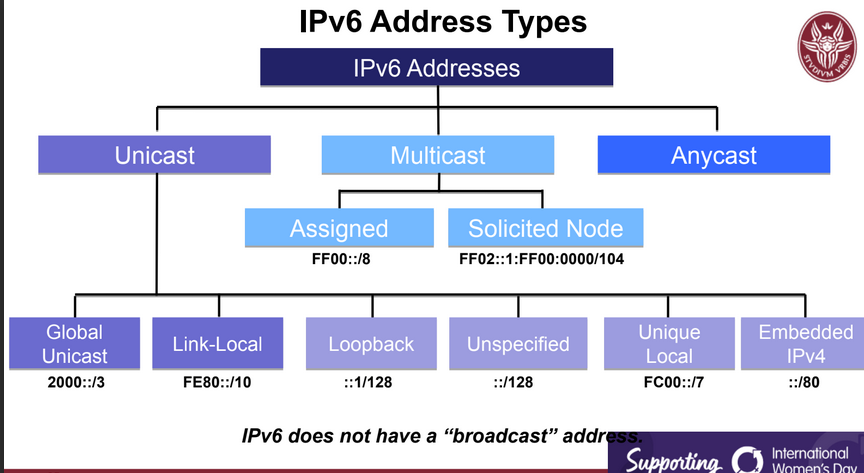
\includegraphics[width=\linewidth]{Include/Chapters/ipv6.PNG}
        \caption{IPv6 address format}
    \end{minipage}
\end{figure}

\begin{itemize}
    \item IPv6 source: always a unicast (link local or GUA)
    \item IPv6 destination: unicast, multicast, or anycast
    \item Global Unicast Address (GUA): globally routable and reachable on the IPv6 internet. It has the following format: 2000::/3 (first 3 bits are 001). The next 45 bits are the global routing prefix, assigned by IANA to RIRs. The next 16 bits are the subnet ID, used to identify subnets within an organization. The last 64 bits are the interface ID, used to identify an interface on a subnet.
    \item prefix: equivalent to the network address of an IPv4 address
    \item prefix length: equivalent to the subnet mask of an IPv4 address
    \item interface ID: equivalent to the host address of an IPv4 address
\end{itemize}

\subsection{Link-local addresses}
Used to comunicate with other devices on the link. Not routable off the link, only have to be unique on the link. Not included in the IPv6 routing table. An ipv6 devise has at least one local link address.

The router link local is used as the default gateway. Routers exchange routing messages and use the link local address as next hop address in the routing

\subsection{SLAAC}
Stateless Address Autoconfiguration (SLAAC) allows a host to 
automatically configure its own IPv6 address without the need
for a DHCP server. The host generates its own interface ID and
combines it with the network prefix obtained from the router 
advertisement messages to create a unique IPv6 address.

The idea is to rovide additional addresses with short lifetime and using themm as source address when 
originating connections. Same prefix as a ublic address, randomized value for interface ID.
It is common to have multiple temporary addresses to make sure existing connections
continue while a new temp address is created for a new connection.



\subsection{ICMPv6 neighbor discover protocol}
ICMPv6 Neighbor Discovery defines 5 different packet types:


\begin{itemize}
    \item Router Solicitation Message
    \item Router Advertisement Message
    \item Neighbor Solicitation Message
    \item Neighbor Advertisement Message
    \item Redirect Message
\end{itemize}

When a host want an IPv6 address, it sends a Router Solicitation message to the all-routers multicast address. The router responds with a Router Advertisement message-
There are 3 types of Router Advertisement messages:
\begin{itemize}
    \item Option 1: SLAAC, No DHCPv6 “I’m everything you need (Prefix, Prefix-length, Default Gateway)”
    \item Option 2: SLAAC + Stateless DHCPv6 for DNS address “Here is my information but you need to get other information such as DNS
            addresses from a DHCPv6 server.” (DNS can be in RA)
    \item Option 3: All addressing except default gateway use DHCPv6
“I can’t help you. Ask a DHCPv6 server for all your information.”
\end{itemize}

\subsection{multicast addresses}
Multicast addresses are used to send a packet to multiple destination simultaneously.
There are two types of multicast addresses: Assigned and Solicited-node.

Multicast address have the prefix FF00::/8. they use a 4 bits field to define the range of the multicast packet, called scope:
\begin{itemize}
    \item 0: reserved
    \item 1: interface-local scope (packets are only valid on the same interface)
    \item 2: link-local scope (packets are only valid on the same link
    \item 5: site-local scope (packets are only valid within the same site)
    \item 8: organization-local scope (packets are only valid within the same organization)
    \item E: global scope (packets are valid on the entire internet)
\end{itemize}

4 bits are used to define the flags:
\begin{itemize}
    \item 0: permnent, well known multicast address 
    \item 1: transient, dynamically assigned multicast address
\end{itemize}

\chapter{IPv4 vs IPv6}
\begin{itemize}
    \item version: Ipv4 contains 4, IPv6 contains 6
    \item internet header lenght(IHL): ipv4 has a 32 bit field including any options or padding, ipv6 has no IHL, his header is fixed at 40bytes
    \item ipv4 has "type of service" field, ipv6 has "traffic class" field 
    \item ipv6 has "flow label" field to identify packets in common stream or flow, ipv4 has no equivalent
    \item ipv4 has 16 bit "total length" field, ipv6 has 32 bit "payload length" field
    \item ipv4 uses fragmentation, ipv6 does not use fragmentation, the source host is responsible for fragmentation
    \item ipv4 protocol, ipv6 next header
    \item ipv4 TTL, ipv6 hop limit
    \item ipv4 header checksum, ipv6 has no header checksum
    \item ipv4 has options and padding, ipv6 has extension headers.  Next headers identify the protoco carried in the data portion of the packet 
\end{itemize}


\section{IPv6 security}
IPv6 is not more secure than IPv4 and its security is built in. Even if there is no NAT  in IPv6, it is possible to use firewalls to filter traffic and you are not exposed to attacks from the internet.
IPv6 is resilient aganinst brute force scanning, but there are other scanning techniques.

There are lots of threats to IPv6, such as:
\begin{itemize}
    \item IP spoofing: using a fake ip source address. Solution: ingress filtering, egress filtering, unicast reverse path forwarding (uRPF)
    \item using traffic clas or flow label to bypass security devices. Solution: firewall should inspect traffic class and flow label fields
    \item routhing header(Includes one or more IPs that should be “visited” in the path) attacks: using extension headers to bypass security devices. Solution: firewall should inspect extension headers
    \item fragmentation attacks: using fragmentation to bypass security devices. Solution: firewall should inspect fragments and reassemble them before inspection
\end{itemize}

\section{associated protocols}
\subsection{ICMPv6}
Provides error messages and informational messages. It is used for error reporting, diagnostics, and neighbor discovery. It is an integral part of the IPv6 protocol suite and is used for various functions such as path MTU discovery, router advertisement, and neighbor solicitation.


\begin{figure}[H]
    \centering
    \begin{minipage}{1\textwidth}
        \centering
        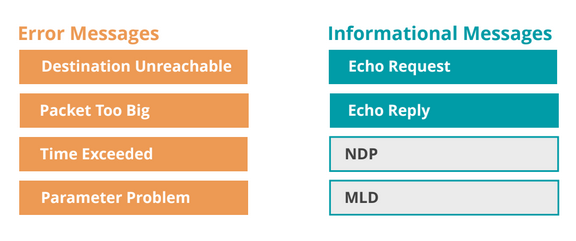
\includegraphics[width=\linewidth]{Include/Chapters/icmpv6.PNG}
        \caption{ICMPv6 message types}\label{fig:icmpv6}
    \end{minipage}
\end{figure}

\subsection{NDP}
Used on a link to discover other devices, their link-layer addresses, and to maintain reachability information about the paths to active neighbors. It is used for address autoconfiguration, address resolution, neighbor unreachability detection, and router discovery.

NDP threats include:
\begin{itemize}
    \item Neighbor solicitation/advertisement spoofing: an attacker can send fake neighbor solicitation or advertisement messages to redirect traffic or cause a denial of service. Solution: use secure neighbor discovery (SEND) which uses cryptographic methods to authenticate messages.
    \item Redirection/DOS attacks: an attacker can send fake redirection messages to redirect traffic or cause a denial of service. Solution: use SEND to authenticate messages.
    \item Man-in-the-middle attacks: an attacker can intercept and modify neighbor discovery messages to redirect traffic or cause a denial of service. Solution: use SEND to authenticate messages.
\end{itemize}

\subsection{MLD}
MLD (multicast listener discovery) is used on local link, uses ICMP, required by NDP. IPv6 nodes use it when joining a multicast group

\chapter{Traffic regulations}
\section{Firewalls}
A firewall is a device that acts like a router and implements rules to determine if packets are allowed to travel from one network to another. they restrict access from outside
prevents attackers from getting too close and restrict people from leaving. To attain a certain level of security you can: regulate traffic allowed, protect
the traffic using encryption, monitor traffic and hosts for "bad behaviour".

firewalls rules/proprieties:
\begin{itemize}
    \item Least privilege
    \item Defense in depth
    \item choke point
    \item weakest links
    \item fail-safe stance
    \item universal partecipation
    \item diversity of defense
    \item simplicity
\end{itemize}

\subsection{Host based packet filters}
A kind of firewall that disciplines traffic in/out a single host, specifies the packets that can be received and sent. Usually each installed application has a known policy that has to obey

\subsection{Network access control list}
Lists the rights for accessing or using networks (used in routers, switches and firewalls). Usually distinguish between incoming
and outgoing traffic, per interface/port. Each packet is treated independently, without any knowledge of what
has come before.

\subsection{Bastion host}
hardened computer used to deal with all traffic coming a protected network from the outside.
Hardening is the task of re reducing or removing vulnerabilities in a computer system:
\begin{itemize}
    \item remove unnecessary software
    \item remove unnecessary services
    \item remove unnecessary accounts
    \item apply patches and updates
    \item use strong authentication and access control
    \item use encryption to protect data in transit and at rest
    \item monitor and log activity on the system
\end{itemize}

\subsection{DMZ}
DMZ stands for demilitarized zone: Computer host or small network inserted as a neutral xone
between a company private network and the outside public network. Network construct that provides secure segregation of networks that host services for users visitors or partners.
DMZ is a necessary method of providing a multilayered defense in depth approch to security. It reduces and regulate
the access to internal(private) components of the IT system.

\subsection{defense in depth}
A security approach in wich IT systems are protected using multiple overlapping systems. It adds redundancy to the defensive measures, it aims to remove single point of failures
it finds the right balance between complexity and multiplicity of defense mechanism. In order to compromise a system, an attacker has to find multiple vulnerabilities in different components.

\subsection{Packet filers (stateless firewalls)}
Drop packets based on source/destination addresses or port numbers or flag. Can operate
on incoming and outgoing traffic. It checks packets with fake id addresses. It operates in data link, network and transport layer.
Problem with packet filters:
\begin{itemize}
    \item Only a small numbers of parameters: it's easy to specify filtering rules that are too specific or too general
    \item Payload of TCP is not inspected: there is no protection against attacks based on upper level vulnerabilities.
    \item limited logging ability
    \item no authentication facilities
    \item suscetible to attacks based on vulnerabilities in various implementation of TCP/IP
\end{itemize}

\subsection{Statefull firewalls}
statefull inspection firewalls can keep track of established connections. Thet can drop packets
based on their source or destination IP addresses, port numbers and TCP flags. In this way they solve
one major problem of simple packet filters, since they can check that incoming traffic from a high-numbered port is a 
genuine response to an outgoing request. 
It operates in data link, network and transoprt level.

\subsection{Application level filtering (proxy-like)}
Deals with the details of services. Needs a separate special purpose mechanism for each application
Can support user to gateway authentication.

\subsection{Host based firewalls}
A firewall on each individual host to protect that one machine. Selectively enable specific services or ports that will be used to send and recive raffic.
It plays a big part in reducing what is accessible from outside and protecting the other element of the system if one is compromised.

\subsection{Circuit level gateways (proxy)}
Also known as TCP relay. The clients connect to a proxy that relays its connection in a protocol independent manner.
Provides user authentication. Usually with no content filtering.

TCP relay splices and relay TCP connection. It does not examine content of TCP segments, can use ACL(like packet filtering) and has less controll than application level gateway.

\chapter{NAT}
NAT (Network address translation) translate the address, connecting a LAN to the internet using un-routable in-house LAN addresses.
In a routed firewall, NAT can filter request from hosts on WAN side to hosts in LAN side, allows host rewuest from LAN side to reach WAN side, and hide LAN host to external port scan.

Routable addresses have to be unique on the internet to be reachable. Non routable addresses are not reachable from the internet.

NAT goals:
\begin{itemize}
    \item a private network uses just one IP address provided by ISP to connect to the internet
    \item private network use private IP addresses provided by IETF
    \item can change address of devices in private network without notifyng outside world
    \item can changhe ISP without changing the addresses of devices in prvate network
    \item Devies inside private network are not explicitly addressable by external network, or visible by outside world.
\end{itemize}

\section{Source NAT (SNAT)}
translate outgoing IP source packet headers from the internal host addresses to the WAN ip address. The session
is masqueraded as coming from NAT device.

The firewall/router forwards replies from the client service request by the external server to the client. Enables the client-server session or connection to continue
on another port as requested by the extrnal server, forwarding any responses by the server to the client.

The NAT table is where associations between request and internal IP addresses are kept.

\section{Basic NAT}
a block of external/public IP addresses are set aside for translating the addresses of hosts within a private domain as they originate sessions to the external domain. 
However, ultiple IP address are difficult to obtain.

\section{Network address port translation (NAPT)}
Multiplex a number of private hosts into a single external/public IP address.
The IP address binding extends to transport level identifiers such as TCP/UDP ports.
NAPT router blocks all incoming ports by default. Many application have had problems with NAPT in their handling of incoming request.

\section{Destination NAT (DNAT)}
Enables destination servers inside a firewall or router LAN to be accessed by clients located outside.
The service appears to be hosted by the firewall/router.

The firewall/router uses NAT table to: Translate incoming packets from
the firewall/router WAN IP address
to the internal address of the
server. Forward the replies to the client
service request from the internal
server to the external client. Enables the client-server session
or connection to continue on
another port as requested by the
internal server, forwarding any
responses by the client to the
server 

\chapter{Iptables}
Foundamentals: 
\begin{itemize}
    \item rules are grouped in "tables"
    \item Each table has different "chains" of rules and different possible "targets"
    \item Each packet is subjected to each rule of a chain
    \item packet fates depend on first matching rule 
\end{itemize}

Built in tables:
\begin{itemize}
    \item filter: default table, used for filtering packets
    \item nat: used for network address translation
    \item mangle: used for specialized packet alteration
    \item raw: used for configuring exemptions from connection tracking
\end{itemize}

\subsection{MANGLE}
Used for IP header manipulation (should not be used for filtering or NAT).
Five chain to alter
\begin{itemize}
    \item PREROUTING: for altering incoming packets before routing
    \item INPUT: for altering packets destined for local sockets
    \item FORWARD: for altering packets being routed through the box
    \item OUTPUT: for altering locally generated packets before routing
    \item POSTROUTING: for altering packets as they are about to go out
\end{itemize}

\subsection{FILTER}
Used for filterning packets. Three built in chains:
\begin{itemize}
    \item INPUT: for packets destined for local sockets
    \item FORWARD: for packets being routed through the box
    \item OUTPUT: for locally generated packets
\end{itemize}

\subsection{NAT}
Used for NAT to translate the packets source field or destination field. (only the first packet of a stream will hit this table, the others will have the same action)

Special targets:
\begin{itemize}
    \item DNAT: for altering destination IP address (PREROUTING and OUTPUT)
    \item SNAT: for altering source IP address (POSTROUTING)
    \item MASQUERADE: for dynamic SNAT (POSTROUTING)
    \item REDIRECT: for altering destination IP to localhost (PREROUTING)
\end{itemize}

\chapter{VPN}
A virtual network built on top of another network infrastructure, wich can provid a secure
comunication mechanism for data and other information transferred between two endpoints. 
Usually based on the use of encryption.

It has the following safety goals:
\begin{itemize}
    \item confidentiality: protect data from unauthorized access
    \item integrity: ensure that data is not tampered with during transmission
    \item authentication: verify the identity of the parties involved in the communication
    \item replay protection: prevent attackers from intercepting and reusing data packets
    \item access control: restrict access to the VPN network to authorized users only
    \item traffic analyis resistance: make it difficult for attackers to analyze the traffic patterns of the VPN network
\end{itemize}

It has the following usability goals:
\begin{itemize}
    \item Transparency: the VPN should be transparent to users and applications, allowing them to use the network as they normally would without any special configuration or changes.
    \item flexibility: the VPN should be flexible enough to support a wide range of use cases and network configurations, including remote access, site-to-site connectivity, and cloud-based deployments.
    \item simplicity: the VPN should be easy to set up and manage, with a user-friendly interface and clear documentation.
\end{itemize}

\section{Tunneling}
Operation of a network connection on top of another network connection, allows two host or sites to communicate through another network that they do not want to use directly.
\subsection{site-to-site tunneling}
Enables a PDU to be transported from one site to another without its content
being processed by hosts on the route. The idea is to incapsulate the whole PDU in another PDU sent out on the network connecting the two sites.
This host-to-host communication does not need to use IP

\subsection{Tunneling for VPN}
tunneling offers the basic methods for providing VPN.
There are two main VPN modes:
\begin{itemize}
    \item split tunneling: Some traffic goes through tunnel, other traffic uses remote user’s default gateway
    \item full tunneling: All traffic goes through tunnel
\end{itemize}

\section{VPN device placement}
\subsection{SSL VPN device placement}
Device placement is a challenge because it affects security, functionality and performance.
The main options for placement are:
\begin{itemize}
    \item VPN functionality on the firewall: VPN functionality is integrated into the firewall, providing a single point of management and security. However, this can create a single point of failure and may not be suitable for high-traffic environments.
    \item VPN device in internal network: The VPN device is placed within the internal network, providing better performance and security. However, this can create a potential security risk if the VPN device is compromised.
    \item Single interface VPN device in DMZ: The VPN device is placed in the DMZ, providing a balance between security and performance. However, this can create a potential security risk if the VPN device is compromised.
    \item Dual interface VPN device in DMZ: The VPN device is placed in the DMZ with two interfaces, providing better security and performance. However, this can create a potential security risk if the VPN device is compromised.
\end{itemize}

\subsection{VPN enabled firewall}
The VPN device communicates directly with internal hosts.

Advantages:
\begin{itemize}
    \item NO holes in FW between VPN device and internal hosts
    \item Traffic between device and internal network must go through FW.
    \item simple network administration since only one box to administer
\end{itemize}
Disadvantages:
\begin{itemize}
    \item Limited to VPN functionality offered by FW vendor.
    \item FW directly accessible to external users via port 443.
    \item Adding VPN functionality to FW can introduce vulnerabilities.
\end{itemize}

\subsection{VPN internal}
Advantages:
\begin{itemize}
    \item Only single rule for single address to be added to FW.
    \item No “holes” needed in FW between VPN device and internal network.
    \item VPN traffic is behind FW, so protected from attacks by machines in DMZ.
\end{itemize}
Disadvantages:
\begin{itemize}
    \item VPN traffic passes through FW on tunnel, so it is not analyzed.
    \item Unsolicited traffic can be sent into internal network from outside to internal
VPN device.
    \item  Internal network is compromised if VPN device is compromised
\end{itemize}

\subsection{DMZ with VPN}
Advantages:
\begin{itemize}
    \item Internal network protected against compromised VPN device.
    \item Traffic between device and internal network must go through FW.
    \item IDS in DMZ can analyze traffic destined for internal network.
\end{itemize}
Disadvantages:
\begin{itemize}
    \item Numerous ports open in FW between device and internal hosts.
    \item Decrypted traffic from device to internal network must be sent through DMZ.
    \item  FW bypassed when user traffic is destined for hosts in DMZ.
\end{itemize}

\subsection{VPN with two interfaces in DMZ}
Clients connect to external device interface, internal traffic uses internal
interface.

Advantages:
\begin{itemize}
    \item All advantages of placing VPN device DMZ.
    \item Unencrypted traffic to internal hosts is protected from other hosts in DMZ.
    \item Only FW interface connected to device’s internal interface needs to permit traffic
from VPN device.
\end{itemize}
Disadvantages:
\begin{itemize}
    \item Numerous ports open in FW between device and internal hosts.
    \item May introduce additional routing complexity.
    \item FW bypassed if split tunneling is not used and user traffic is destined for hosts in
DMZ
\end{itemize}

\section{SSL tunneling}
\subsection{SSL e TLS}
Secure sockets layer (SSL) and transport layer security (TLS) are one of the most
widely used security services.General-purpose service
implemented as a set of
protocols that rely on TCP.
SSL applies security in the transport layer, placed on top of TCP, so no need to change TCP/IP stack or OS.
Provides secure channel. Optional server authentication with public key certificates.

\subsection{SSL protocol architectures} 
Adds extra layer between T and A layer, adding extra elements to A layer.

Record Protocol: Protocol offering
basic encryption and integrity
services to applications

Application Protocols: control operation
of the record protocol: Handshake: Used to authenticate server (and optionally client) and to agree on
encryption keys and algorithms. Change cipher spec: Selects agreed keys and encryption algorithm until further
notice. Alert: Transfers information about failures.

\subsection{SSL/TLS Handshake protocol}
4 phases:
\begin{itemize}
    \item Hello: Establishment of security capabilities: Client sends list of possibilities, in
order of preference. Server selects one, and informs Client of its choice. Parties also
exchange random noise for use in key generation.
 \item Server authentication and key exchange: Server executes selected key exchange
protocol (if needed). Server sends authentication info. (e.g. X.509 cert.) to Client.
\item Client authentication and key exchange: Client executes selected key exchange
protocol (mandatory). Client sends authentication info. to Server (optional).
\item Finish: Shared secret key is derived from pre-secrets exch. in 2, 3. Change Cipher
Spec. protocol is activated. Summaries of progress of Handshake Protocol are
exchanged and checked by both parties.
\end{itemize}

\subsection{Digital certificate and certification authorities}
digital certificate are documents that certifie the relation between a public
key and its owner. to verify them we need a public key that we trust. 
Trusted public keys are stored in certificates of certification authorities (CA).
CA are organizations that issue digital certificates and perform vary task, such as:
\begin{itemize}
    \item Receive application for keys.
    \item Verify applicant’s identity, conduct due diligence appropriate to the trust level,
and issue key pairs.
    \item Store public keys and protect them from unauthorized modification.
    \item Keep a register of valid keys.
    \item Revoke and delete keys that are invalid or expired. Maintain a certificate
revocation list (CRL).

\end{itemize}
Certificates of CAs are stored in any computer that want to use internet
securely.

Certification authorities are
organized in a hierarchy, called
Public Key Infrastructure. To verify a certificate, one needs
to verify all the signatures up to
the top of the hierarchy

\subsection{SSL/TSL heartbeat}
It is an extension (RFC 6520) that allows to keep an established session
alive
To avoid the re-negotiation of the security parameters for establishing a
secure session, we can keep using the same parameters even if there is
no exchange of data
It introduces two messages: HeartbeatRequest and HeartbeatResponse
When one endpoint sends a HeartbeatRequest message to the other
endpoints, the former also starts what is known as the retransmit timer
 An SSL/TLS session is considered to have terminated in the absence of a
HeartbeatResponse packet within a time interval.
As a protection against a replay attack, HeartbeatRequest packets
include a payload that must be returned without change by the receiver
in its HeartbeatResponse packet.